\chapter{Paralelní výpočty}

V této kapitole proberu úvod do využívání paralelních počítačů.

\section{Sériové vs. paralelní výpočty}

Podívejme se například na následující pseudokód.

\begin{Verbatim}
for(i=0;i<N;i++){
  	resultA	= task_a(i);
   	resultB	= task_b(i);
   	resultC	= task_c(i);
   	resultD	= task_d(i);
   	resultAll	+= resultA + resultB + resultC + resultD;
}    
\end{Verbatim}

Provádění výše uvedeného kódu na jednom jednojádrovém procesoru znamená, že budeme muset
provést \emph{task\_a}, pak \emph{task\_b}, následně \emph{task\_c} a nakonec \emph{task\_d}.
To vše je třeba udělat $N$ krát. Pro případ $N=4$ platí obrázek \ref{obr:serialvspara}. Tomuto případu říkáme \emph{sériový přístup}.

Nyní ale máme k dispozici dvoujádrový procesor. Bez problémů na něm můžeme spustit výše uvedený program. Druhé jádro tohoto nového dvoujádrového procesoru je ale zcela nevytíženo. Výpočet je tak do značné míry neefektivní. Řešením by tedy bylo, aby úkol byl rozdělen na dva poloviční úkoly a na každém jádře by byl prováděn právě jeden. Tomuto říkáme \emph{paralelní přístup} \ref{obr:serialvspara}.

\begin{figure}
  \begin{center}
    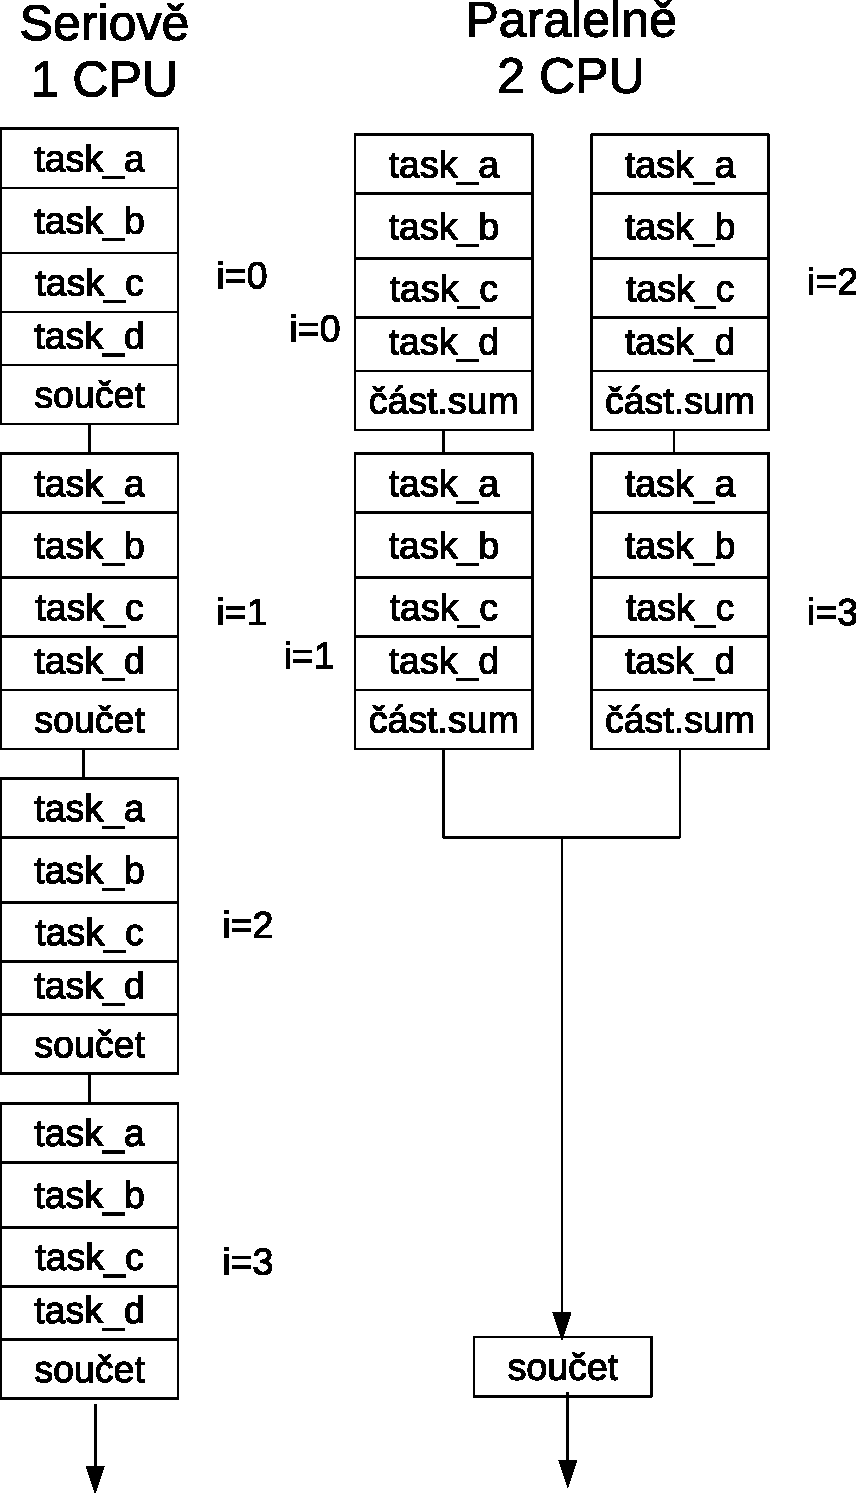
\includegraphics[scale=.6]{obr/serialvspara}
  \end{center}
  \caption{Porovnání sériového a paralelního přístupu}
  \label{obr:serialvspara}
\end{figure}

Během plánovací fáze paralelních programů je třeba vzít v úvahu některé stávající zákony. První zákon říká, že pokud program provádí nějaké \% časového kódu, který nelze provést paralelně, předpokládá se, že očekávaná rychlost z paralelizace bude v nejlepším zlepšení 1 / $y$. Zákon lze prokázat následovně. Předpokládejme, že $T_s$ představuje čas potřebný pro spuštění části kódu, kterou nelze paralelizovat, a $T_p$ představuje čas potřebný pro spuštění části kódu, který může mít prospěch z~paralelizace. Spuštěním programu s 1 procesorem je doba zpracování:

\begin{myequation}
\begin{aligned}
\label{vztah:serialcputimes}
T(1) = T_s + T_p
\end{aligned}
\end{myequation}

Když ale použijeme $N$ procesorů, tak je to méně:

\begin{myequation}
\begin{aligned}
\label{vztah:serialcputimes}
T(N) = T_s + T_p / N
\end{aligned}
\end{myequation}

Pokud řekneme, že $N$ jde do nekonečna, zrychlíme výpočet až $S = 1/y$. Tomuto zákonu se říká \emph{Amdahlův}.
         
\section{Datový paralelismus vs. úlohový paralelismus}

V paralelizaci jsou dva základní přístupy. Jedna instrukce a více dat (SIMD \ref{sec:simd}), které představuje datový paralelismus a Více instrukcí(jedna úloha) více dat (SPMD \ref{sec:spmd}) představující úlohový paralelismus.


\subsection{Datový paralelismus}


Takovým příkladem pro SIMD je sčítání vektorů. Všechny výpočetní jednotky provádějí stejnou instrukcí, každá však nad jiným indexem.


\subsection{Úlohový paralelismus}

Kdyby se však stejný postup místo na instrukce použil na celou úlohu, efektivita výpočtu by se zjevně snížila. Každá úloha by potřebovala jinak dlouhý časový úsek pro svou práci. 

\subsection{Load balancing}

Load balancing je technika, která dokáže využít plně možností víceprocesorového systému. Zde je implementována fronta procesů, ze které se systém postupně odebírá a přiděluje tak procesy volným jádrům.

\subsection{Pipeline}

\begin{figure}
  \begin{center}
    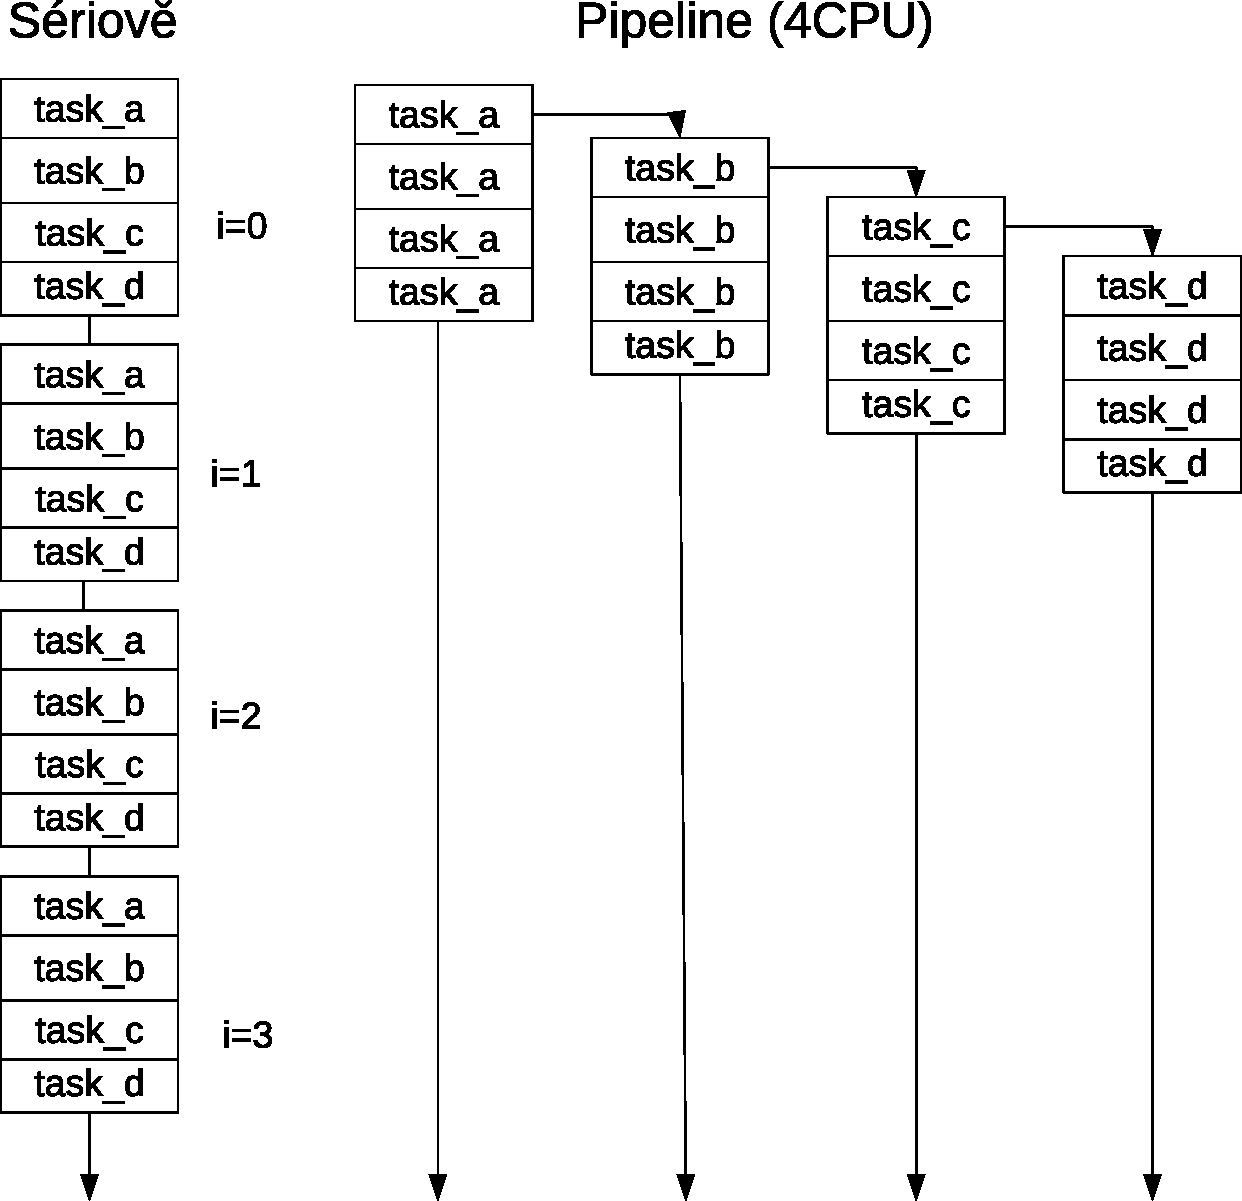
\includegraphics[scale=.6]{obr/pipeline}
  \end{center}
  \caption{Porovnání sériového přístupu a pipeline}
  \label{obr:serialvspipeline}
\end{figure}

Obrázek \ref{obr:serialvspipeline} ukazuje, že je možný ještě další přístup. Každý procesor je specializovaný na jednu určitou úlohu. Toto schema se s výhodou využívá
například u zpracování videa či signálů. 